% docs/architecture.tex
% Architecture of the project: a reusable LLM/RAG evaluation framework,
% demonstrated on an AI & Technology News Assistant.
%
% Build (any TeX distribution with TikZ):
%     pdflatex architecture.tex
% or paste into Overleaf. Produces a single-page PDF.

\documentclass{article}
\usepackage[a4paper,margin=12mm]{geometry}
\pagestyle{empty}
\usepackage{tikz}
\usepackage[T1]{fontenc}
\usepackage{helvet}
\renewcommand{\familydefault}{\sfdefault}
\usetikzlibrary{arrows.meta,positioning,fit,backgrounds,calc}

\begin{document}
\begin{center}
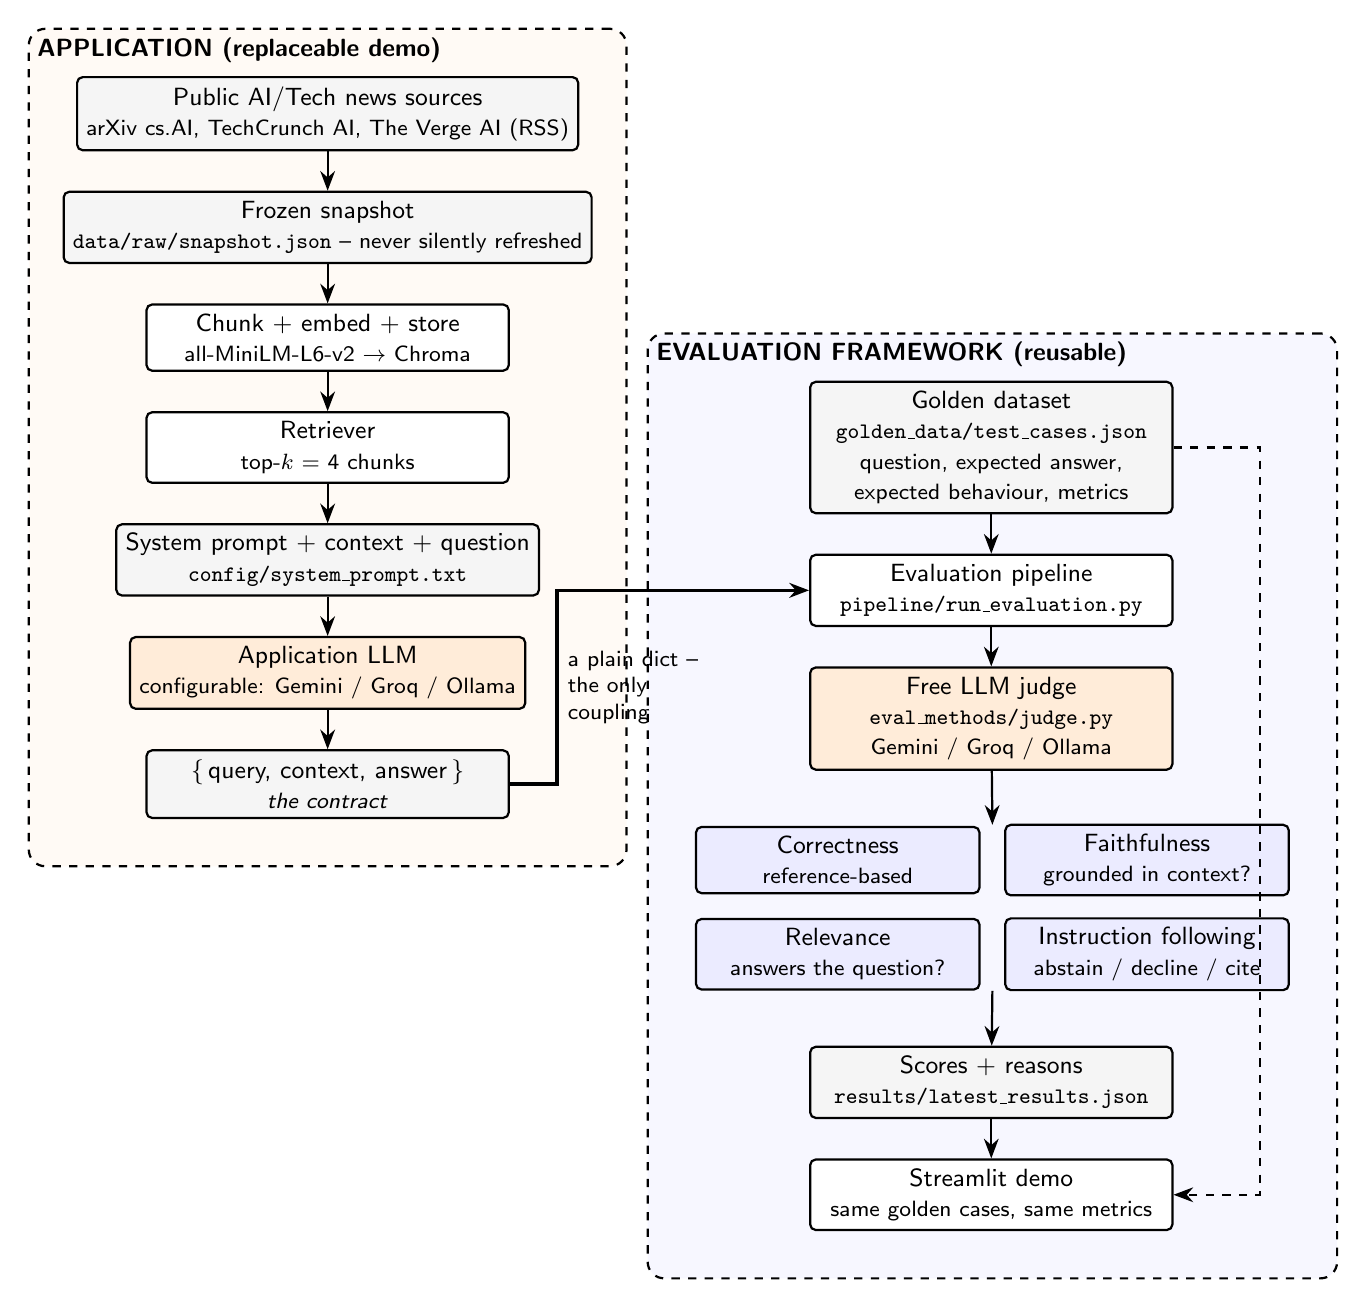
\begin{tikzpicture}[
    font=\small,
    node distance=5mm and 12mm,
    box/.style={draw, rounded corners=2pt, minimum width=46mm, minimum height=8mm,
                align=center, fill=white, thick},
    data/.style={box, fill=gray!8},
    llm/.style={box, fill=orange!15},
    metric/.style={draw, rounded corners=2pt, minimum width=36mm, minimum height=8mm,
                   align=center, fill=blue!8, thick},
    flow/.style={-{Stealth[length=2.5mm]}, thick},
    region/.style={draw, dashed, rounded corners=6pt, inner sep=6mm, thick},
    label/.style={font=\bfseries\small, anchor=north west},
]

% =====================  APPLICATION  =====================
\node[data]                       (sources) {Public AI/Tech news sources\\{\footnotesize arXiv cs.AI, TechCrunch AI, The Verge AI (RSS)}};
\node[data,  below=of sources]    (snap)    {Frozen snapshot\\{\footnotesize \texttt{data/raw/snapshot.json} -- never silently refreshed}};
\node[box,   below=of snap]       (kb)      {Chunk + embed + store\\{\footnotesize all-MiniLM-L6-v2 $\rightarrow$ Chroma}};
\node[box,   below=of kb]         (retr)    {Retriever\\{\footnotesize top-$k$ = 4 chunks}};
\node[data,  below=of retr]       (prompt)  {System prompt + context + question\\{\footnotesize \texttt{config/system\_prompt.txt}}};
\node[llm,   below=of prompt]     (appllm)  {Application LLM\\{\footnotesize configurable: Gemini / Groq / Ollama}};
\node[data,  below=of appllm]     (answer)  {\{\,query, context, answer\,\}\\{\footnotesize \textit{the contract}}};

\draw[flow] (sources) -- (snap);
\draw[flow] (snap)    -- (kb);
\draw[flow] (kb)      -- (retr);
\draw[flow] (retr)    -- (prompt);
\draw[flow] (prompt)  -- (appllm);
\draw[flow] (appllm)  -- (answer);

\begin{scope}[on background layer]
  \node[region, fit=(sources)(answer), fill=orange!4] (appregion) {};
\end{scope}
\node[label] at (appregion.north west) {APPLICATION (replaceable demo)};

% =====================  EVALUATION FRAMEWORK  =====================
\node[data,  right=38mm of retr]   (golden)  {Golden dataset\\{\footnotesize \texttt{golden\_data/test\_cases.json}}\\{\footnotesize question, expected answer,}\\{\footnotesize expected behaviour, metrics}};
\node[box,   below=of golden]      (runner)  {Evaluation pipeline\\{\footnotesize \texttt{pipeline/run\_evaluation.py}}};
\node[llm,   below=of runner]      (judge)   {Free LLM judge\\{\footnotesize \texttt{eval\_methods/judge.py}}\\{\footnotesize Gemini / Groq / Ollama}};

% the four metrics
\node[metric, below=7mm of judge, xshift=-19.5mm] (m1) {Correctness\\{\footnotesize reference-based}};
\node[metric, right=3mm of m1]                  (m2) {Faithfulness\\{\footnotesize grounded in context?}};
\node[metric, below=3mm of m1]                  (m3) {Relevance\\{\footnotesize answers the question?}};
\node[metric, right=3mm of m3]                  (m4) {Instruction following\\{\footnotesize abstain / decline / cite}};

\node[data,  below=7mm of m3, xshift=19.5mm] (scores) {Scores + reasons\\{\footnotesize \texttt{results/latest\_results.json}}};
\node[box,   below=of scores]              (ui)     {Streamlit demo\\{\footnotesize same golden cases, same metrics}};

\draw[flow] (golden) -- (runner);
\draw[flow] (runner) -- (judge);
\draw[flow] (judge)  -- ($(m1.north)!0.5!(m2.north)$);
\draw[flow] ($(m3.south)!0.5!(m4.south)$) -- (scores);
\draw[flow] (scores) -- (ui);

\begin{scope}[on background layer]
  \node[region, fit=(golden)(m1)(m4)(ui), fill=blue!3] (evalregion) {};
\end{scope}
\node[label] at (evalregion.north west) {EVALUATION FRAMEWORK (reusable)};

% the only connection between the two halves
\draw[flow, very thick]
  (answer.east) -- ++(6mm,0) |- (runner.west)
  node[pos=0.25, right, align=left, font=\footnotesize]
  {a plain dict --\\the only\\coupling};

% golden data feeds the demo directly too
\draw[flow, dashed] (golden.east) -- ++(11mm,0) |- (ui.east);

\end{tikzpicture}
\end{center}
\end{document}
